\documentclass{beamer}

\usetheme{Boadilla}

% Title
\title{Vim Lab}
\author{Ethan Wong}
\date{October 13, 2023}
\institute{Linux Users Group @ UIC}

\begin{document}

\begin{frame}
	\titlepage
\end{frame}

\begin{frame}{Table of Contents}
	\tableofcontents[pausesections]
\end{frame}

\section{Why Vim?}
\begin{frame}{Why Vim?}
	\begin{itemize}
		\item Simple and ubiquitous text editor 
		\item Usable in a \textit{terminal}
		\item Vim's version of modal input is popular and commonly emulated
		\item Part of the POSIX standard!
	\end{itemize}
\end{frame}

\section{History}
\begin{frame}{Table of Contents}
	\tableofcontents[currentsection]
\end{frame}

\begin{frame}{History}
	\begin{columns}
		\begin{column}{0.5\textwidth}
			\begin{itemize}
				\item Vi(no -m) was created by Bill Joy in \textbf{1976} for the
					Second BSD.\footnotemark
					\pause

				\item It is the visual mode for the \texttt{ex}
					command line text editor.
					\pause

				\item Vi was created for remote editing over a \textit{300} baud
					modem, which transmitted text slower than you can read!
					\pause
			\end{itemize}
		\end{column}
		\begin{column}{0.5\textwidth}
			\begin{figure}
				\centering
				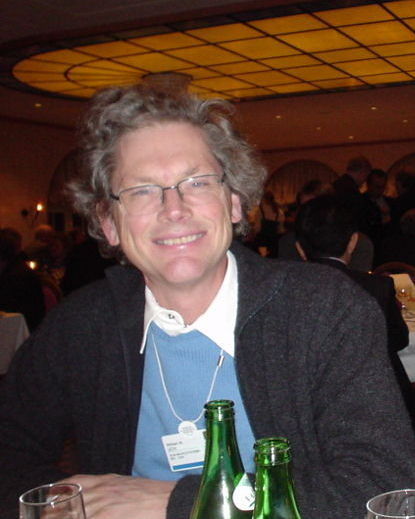
\includegraphics[width=0.5\textwidth]{bill_joy.jpg}
				\caption{Bill Joy, the creator of \texttt{vi}}
			\end{figure}
		\end{column}
	\end{columns}

	\footnotetext{\url{https://web.archive.org/web/20060701083055/http://web.cecs.pdx.edu/~kirkenda/joy84.html}}
\end{frame}

\begin{frame}{History}
	\begin{itemize}
		\item Vi iMproved (\texttt{vim}) was created by Bram Moolenaar
			in 1988 as a \textit{clone} of \texttt{vi}.
			\pause

		\item \texttt{vim} is a superset of \texttt{vi}, introducing new
			features such as syntax highlighting, undo/redo, screen
			splitting, and plugin support.
			\pause

		\item Like \texttt{vi}, \texttt{vim} has also been ported to a
			wide range of OS's.
			\pause

		\item Today, \texttt{vim} and its derivatives
			are one of the most popular text
			editors.\footnotemark
			\pause
	\end{itemize}

	\footnotetext{\url{https://survey.stackoverflow.co/2023/\#section-most-popular-technologies-integrated-development-environment}}
\end{frame}


\section{Basic Knowledge}
\begin{frame}{Table of Contents}
	\tableofcontents[currentsection]
\end{frame}

\begin{frame}{Basic Knowledge}
	\texttt{vim} is known for 
\end{frame}

\section{Crash Course}
\begin{frame}{Table of Contents}
	\tableofcontents[currentsection]
\end{frame}

\end{document}

% vim: set tw=80:
